%%%%%%%%%%%%%%%%%%%%%%%%%%%%%%%%%%%%%%%%%
% Beamer Presentation
% LaTeX Template
% Version 1.0 (10/11/12)
%
% This template has been downloaded from:
% http://www.LaTeXTemplates.com
%
% License:
% CC BY-NC-SA 3.0 (http://creativecommons.org/licenses/by-nc-sa/3.0/)
%
%%%%%%%%%%%%%%%%%%%%%%%%%%%%%%%%%%%%%%%%%

%----------------------------------------------------------------------------------------
%	PACKAGES AND THEMES
%----------------------------------------------------------------------------------------

\documentclass{beamer}

\mode<presentation> {

% The Beamer class comes with a number of default slide themes
% which change the colors and layouts of slides. Below this is a list
% of all the themes, uncomment each in turn to see what they look like.

%\usetheme{default}
%\usetheme{AnnArbor}
%\usetheme{Antibes}
%\usetheme{Bergen}
%\usetheme{Berkeley}
%\usetheme{Berlin}
%\usetheme{Boadilla} % sieht nett aus
%\usetheme{CambridgeUS}
%\usetheme{Copenhagen}
%\usetheme{Darmstadt}
%\usetheme{Dresden}
%\usetheme{Frankfurt}
%\usetheme{Goettingen}
%\usetheme{Hannover} % sieht nett aus
%\usetheme{Ilmenau}
%\usetheme{JuanLesPins}
%\usetheme{Luebeck}
\usetheme{Madrid}
%\usetheme{Malmoe}
%\usetheme{Marburg}
%\usetheme{Montpellier}
%\usetheme{PaloAlto}
%\usetheme{Pittsburgh}
%\usetheme{Rochester}
%\usetheme{Singapore}
%\usetheme{Szeged}
%\usetheme{Warsaw}

% As well as themes, the Beamer class has a number of color themes
% for any slide theme. Uncomment each of these in turn to see how it
% changes the colors of your current slide theme.

%\colorlet{beamer@blendedblue}{green!25!black} % Influence color of Theme here!
%\usecolortheme{albatross}
%\usecolortheme{beaver}
%\usecolortheme{beetle}
%\usecolortheme{crane}
%\usecolortheme{dolphin}
%\usecolortheme{dove}
%\usecolortheme{fly}
%\usecolortheme{lily}
%\usecolortheme{orchid}
%\usecolortheme{rose}
%\usecolortheme{seagull}
%\usecolortheme{seahorse}
%\usecolortheme{whale}
%\usecolortheme{wolverine}

%\setbeamertemplate{footline} % To remove the footer line in all slides uncomment this line
%\setbeamertemplate{footline}[page number] % To replace the footer line in all slides with a simple slide count uncomment this line

\setbeamertemplate{navigation symbols}{} % To remove the navigation symbols from the bottom of all slides uncomment this line
}

\usepackage{color}

\PassOptionsToPackage{table,svgnames,dvipsnames}{xcolor}

%\usepackage[autostyle]{csquotes}
\usepackage[%  
  backend=bibtex,
  url=false,
  style=authoryear,
  maxnames=2,
  minnames=1,
  maxbibnames=99,
  firstinits,
  hyperref=true,
  doi=false,
  isbn=false,
  url=false,
  eprint=false,
  uniquename=init]{biblatex} % TODO: adapt bibliography style
\setlength{\bibnamesep}{0.5\baselineskip}
\renewcommand*{\nameyeardelim}{\addcomma\space}
\usepackage{graphicx}
\usepackage{lstautogobble}
\usepackage{tikz}
\usetikzlibrary{arrows}
\usetikzlibrary{shapes}
\usetikzlibrary[pgfplots.groupplots]
\usepackage{tikzscale}
\usepackage{pgfplots}
\usepackage{pgfplotstable}
\usepackage{marvosym}
\usepackage{array}
\usepackage{booktabs}
\usepackage{hyperref} % hidelinks removes colored boxes around references and links
\usepackage[textwidth=1.5cm, textsize=tiny]{todonotes}
\usepackage{pdfpages}
\usepackage{lipsum}
\usepackage{amsmath}
\usepackage{mathtools}
\usepackage{amssymb}
\usepackage{amsthm}
\usepackage{algorithm,algpseudocode}
\usepackage[titletoc,toc,title,page]{appendix}
\usepackage{scrhack} % necessary for listings package
\usepackage{listings}

%%%% Allows for checks and x if fulfilled/not fulfilled
\usepackage{pifont}
\newcommand{\cmark}{\ding{51}}%
\newcommand{\xmark}{\ding{55}}%
%%%%

 % Allows for use of textcolor

%%%%% TESTSPACE - Hinterlegung von Gleichungen mit Farbe %%%%%
\usepackage{calc}
\usepackage{xcolor}
\usepackage{color, colortbl}

\newlength\dlf
\newcommand\alignedbox[3][yellow]{
  % #1 = color (optional, defaults to yellow)
  % #2 = before alignment
  % #3 = after alignment
  &
  \begingroup
  \settowidth\dlf{$\displaystyle #2$}
  \addtolength\dlf{\fboxsep+\fboxrule}
  \hspace{-\dlf}
  \fcolorbox{red}{#1}{$\displaystyle #2 #3$}
  \endgroup
}

%%%%% 0TESTSPACE - Änderung des Designs Inhaltsverzeichnis%%%%%

\setbeamertemplate{section in toc}{%
  {\inserttocsectionnumber.}~\inserttocsection}
%\setbeamercolor{subsection in toc}{bg=white,fg=structure}
\setbeamertemplate{subsection in toc}{%
  \hspace{1.2em}{\color{orange}\rule[0.3ex]{3pt}{3pt}}~\inserttocsubsection\par}

	%%%%% TESTSPACE - Änderung des Bulletpointdesigns%%%%%
		\setbeamertemplate{itemize items}{%
		\hspace{1.2em}{\color{orange}\rule[0.3ex]{3pt}{3pt}}~}
		\setbeamertemplate{enumerate items}[default]


%%%%% 1TESTSPACE - Manipulation Footer%%%%%
\makeatletter
\setbeamertemplate{footline}
{
  \leavevmode%
  \hbox{%
  \begin{beamercolorbox}[wd=.333333\paperwidth,ht=2.25ex,dp=1ex,center]{author in head/foot}%
    \usebeamerfont{author in head/foot}\insertsection
  \end{beamercolorbox}%
  \begin{beamercolorbox}[wd=.333333\paperwidth,ht=2.25ex,dp=1ex,center]{title in head/foot}%
    \usebeamerfont{title in head/foot}\insertsubsection
  \end{beamercolorbox}%
  \begin{beamercolorbox}[wd=.333333\paperwidth,ht=2.25ex,dp=1ex,right]{date in head/foot}%
    \usebeamerfont{date in head/foot}%\insertshortdate{}\hspace*{2em}
    \insertframenumber{} \hspace*{2ex} 
  \end{beamercolorbox}}%
  \vskip0pt%
}
\makeatother

%gets rid of bottom navigation bars
\setbeamertemplate{footline}[frame number]{}
%gets rid of navigation symbols
\setbeamertemplate{navigation symbols}{}

%%%%% 2TESTSPACE %%%%% Definiere Abrunden/Aufrunden
\usepackage{mathtools}
\DeclarePairedDelimiter\ceil{\lceil}{\rceil}
\DeclarePairedDelimiter\floor{\lfloor}{\rfloor}

% Math helpers
\newcommand{\E}{\mathbb{E}}
\newcommand{\Var}{\mathrm{Var}}
\newcommand{\Cov}{\mathrm{Cov}}
\newcommand{\tn}{\tabularnewline}

%%%%% 3TESTSPACE %%%%% Manipulation Header
%\definecolor{greyone}{RGB}{77,77,77}
%\setbeamercolor{palette quaternary}{fg=white,bg=greyone!20}
%\setbeamercolor{titlelike}{parent=palette quaternary}
%\setbeamertemplate{frametitle}
%{
%    \nointerlineskip
%    \begin{beamercolorbox}[sep=0.1cm,ht=1.8em,wd=\paperwidth]{frametitle}
%        \vbox{}\vskip-2ex%
%        \raisebox{-3mm}{}
%        \strut\insertframetitle\strut
%        \hfill
%        \vskip-0.9ex%
%    \end{beamercolorbox}
%}
%%%%% 4TESTSPACE %%%%% Manipulation Titelseite
\usepackage{tikz}
\newcommand*{\mytitle}{Production \& Capacity Planning} % Title
\newcommand*{\myauthor}{Christopher Wolf} % Presenters name(s)
\newcommand*{\mydate}{May 27,2015} % Presentation date
\definecolor{mygreen}{RGB}{44,85,17}
\definecolor{myblue}{RGB}{34,31,217}
\newcommand*{\mygreen}[1]{\textcolor{mygreen}{#1}}
%%%%% 5TESTSPACE %%%%% Multicolumn Lists
\usepackage{multicol}

\newcommand{\lenitem}[2][.45\linewidth]{\parbox[t]{#1}{\strut #2\strut}}

\bibliography{bibliography/library}

%----------------------------------------------------------------------------------------
%	TITLE PAGE
%----------------------------------------------------------------------------------------
\title[Short title]{Variational Inference with Hamiltonian Monte Carlo} % The short title appears at the bottom of every slide, the full title is only on the title page

\author{Christopher Wolf} % Your name
\institute[] % Your institution as it will appear on the bottom of every slide, may be shorthand to save space
{Technische Universit\"at M\"unchen  \\ % Your institution for the title page
\medskip
\textit{christopher.wolf@tum.de} % Your email address
}
\date{February 4, 2016} % Date, can be changed to a custom date

\begin{document}

%----------------------------------------------------------------------------------------
%	ALTERNATIVE TITLE PAGE
%----------------------------------------------------------------------------------------

%\begin{frame}[plain]
%% No slide header and footer
%	\begin{tikzpicture}[remember picture,overlay] % Background box
%		\node [xshift=\paperwidth/2,yshift=\paperheight/2] at (current page.south west)[rectangle,fill,inner sep=0pt,minimum width=\paperwidth,minimum height=\paperheight/4,top 				color=myblue!90!black,bottom color=myblue!60!black]{}; % Change the height of the box, its colors and position on the page here
%	\end{tikzpicture}
%% Text within the box
%\begin{flushright}
%	\vspace{1.95cm}
%	\color{white}\sffamily
%	{\bfseries\Large\mytitle\par} % Title
%	\vspace{0.5cm}
%	\normalsize
%	\myauthor\par % Author name
%	%\mydate\par % Date
%	\vfill
%\end{flushright}
%\end{frame}

%----------------------------------------------------------------------------------------
%	NORMAL TITLE PAGE
%----------------------------------------------------------------------------------------

\begin{frame}
\titlepage % Print the title page as the first slide
\end{frame}

%----------------------------------------------------------------------------------------
%	TABLE OF CONTENTS
%----------------------------------------------------------------------------------------

%\begin{frame}
%\frametitle{Overview} % Table of contents slide, comment this block out to remove it
%\tableofcontents % Throughout your presentation, if you choose to use \section{} and \subsection{} commands, these will automatically be printed on this slide as an overview of your presentation
%\end{frame}

%----------------------------------------------------------------------------------------
%	PRESENTATION SLIDES
%----------------------------------------------------------------------------------------

%------------------------------------------------
\section{Introduction} 
%------------------------------------------------
\nocite{Neal2011}
	%------------------------------------------------
	\subsection{Variational inference} 
	%------------------------------------------------
	\begin{frame}
		\frametitle{Variational inference}
		
		\textbf{Setting}: Probabilistic model $p(x, z)$ with missing or latent variables $z$\\~\\
		\begin{itemize}
		\item Quantity of interest: Marginal likelihood $p(x) = \int p(x, z) dz$\\~\\
		\item Often not directly tractable\\~\\
		\item Use a variational lower bound
		\end{itemize}
		\begin{equation*}
		\begin{split}
		\log p(x) &\geq \log p(x) - D_{KL} \left( q_{\theta}(z|x) || p(z|x) \right) \\
					   &=  \E_{q_{\theta}(z|x)} \left[ \log p(x, z) - \log q_\theta(z|x) \right] \eqqcolon \mathcal{L}
		\end{split}
		\end{equation*}\\~\\
		% Beim Erklären der Bound und der involvierten Optimierung: VAE erwähnen
		\uncover<2->{\textbf{Problem}: Quality of the bound strongly depends on the ability of $q_\theta(z|x)$ to approximate the true posterior}\\~\\
		\uncover<3->{\textbf{Aim of this work}: Improve the approximation}
	\end{frame}

	% VI and VAE
	% Problem: Posterior approximation with parameteric family -> limited flexibility -> possibly only bad approximation
	% Aim of this work: Improve flexibility
	% Need to move away from purely parametric approach! Need something, which finds the posterior in a different way!
	
	%------------------------------------------------
	\subsection{MCMC} 
	%------------------------------------------------
	% Idea: Create Markov chain, which converges to the target distribution
	% Most popular: Metropolis-Hastings algorithm -> Acceptance step
	\begin{frame}
		\frametitle{Markov Chain Monte Carlo (MCMC) methods}
		
		\textbf{Objective}: Generate samples from a complicated distribution $f_{\textrm{target}}(s)$\\~\\
		\textbf{Idea}: Create a Markov chain $(s_t)_{t \in \mathbb{N}}$, which converges to the target distribution\\~\\
		\uncover<2->{\textbf{Metropolis-Hastings algorithm}: Produces such a Markov chain
		\begin{enumerate}
			\item Generate a proposal $\tilde{s}$ from some distribution $f_{\textrm{prop}}(\tilde{s}|s_{t-1})$ (with $f_{\textrm{prop}}(t|s) = f_{\textrm{prop}}(s|t)$)
			\item Accept the proposal as the next state $s_t$ with probability
				\begin{equation*}
				p_{\textrm{accept}} = \min[1, \frac{f_{\textrm{target}}(\tilde{s})}{f_{\textrm{target}}(s_{t-1})}],
				\end{equation*}
				otherwise set $s_t = s_{t-1}$.
		\end{enumerate}}
	\end{frame}	
	
	%------------------------------------------------
	\subsection{VI with MCMC} 
	%------------------------------------------------
	\begin{frame}
		\frametitle{Integrating MCMC into variational inference}
		\textcite{Salimans2014}: Interpret the Markov chain obtained in MCMC as a variational approximation \\~\\ %$q(z_0, \dots, z_T|x) = q_{0}(z_0|x) \cdot \prod_{t=1}^T q(z_t|z_{t-1}, x)$
		\textbf{Problem}: Original lower bound $\mathcal{L} = \E_{q(z_T|x)} \left[ \log p(x, z_T) - \log q(z_T|x) \right]$ is now intractable, so it needs to be modified:
		\uncover<2->{\begin{equation*}
		\begin{split}
		\log &p(x) \geq \mathcal{L} \\
	  		&\geq \mathcal{L} - \E_{q(z_T|x)} \big[ D_{KL} \left( q(z_0, \dots, z_{T-1} |z_T, x) || r(z_0, \dots, z_{T-1}|z_T, x) \right) \big] \\
	  		&\eqqcolon \mathcal{L}_{\textrm{aux}},
		\end{split}
		\end{equation*} \\~\\		
		$\boldsymbol{\rightarrow}$ Need to also learn a \textit{reverse} model $r(z_0, \dots, z_{T-1}|z_T, x)$}
		% Training as for basic VI
		% Steps are computationally expensive -> need efficient MCMC method -> HMC		
	\end{frame}	

%------------------------------------------------
\section{Hamiltonian Monte Carlo}
%------------------------------------------------

	%------------------------------------------------
	\subsection{Hamiltonian Dynamics} 
	%------------------------------------------------
	\begin{frame}
		\frametitle{Hamiltonian Dynamics}
		\begin{itemize}
		\item Reformulation of classical dynamics \\~\\ %e.g. Newton's equation of motion)
		\item System state given by \textit{position} $z$ and \textit{momentum} $v$ \\~\\
		\uncover<2->{\item For HMC: Motion of frictionless particle due to \textit{potential energy} $U(z)$ and \textit{kinetic energy} $K(v)$ \\~\\}
		\uncover<3->{\item $U(z) = - \log p(x, z)$, the NLL of $p(z|x)$ upto additive constants \\~\\} % inspired by statistical physics relating energy of a state to its probability density
		\uncover<4->{\item $K(v) = (1/2) v^T M^{-1} v + C= - \log N(v|0, M)$, $M$ called the mass matrix}  % gives the physically intuitive kinetic energy, corresponds to particle mass (important later)
		\end{itemize}
	\end{frame}	

	\begin{frame}
		\frametitle{Hamiltonian Dynamics - Numerical Solution}
		Leapfrog method: 
		\begin{itemize}
			\item volume-preserving
			\item reversible
			\item approximate conservation of total energy\\~\\
		\end{itemize}
		\centering
		\uncover<2->{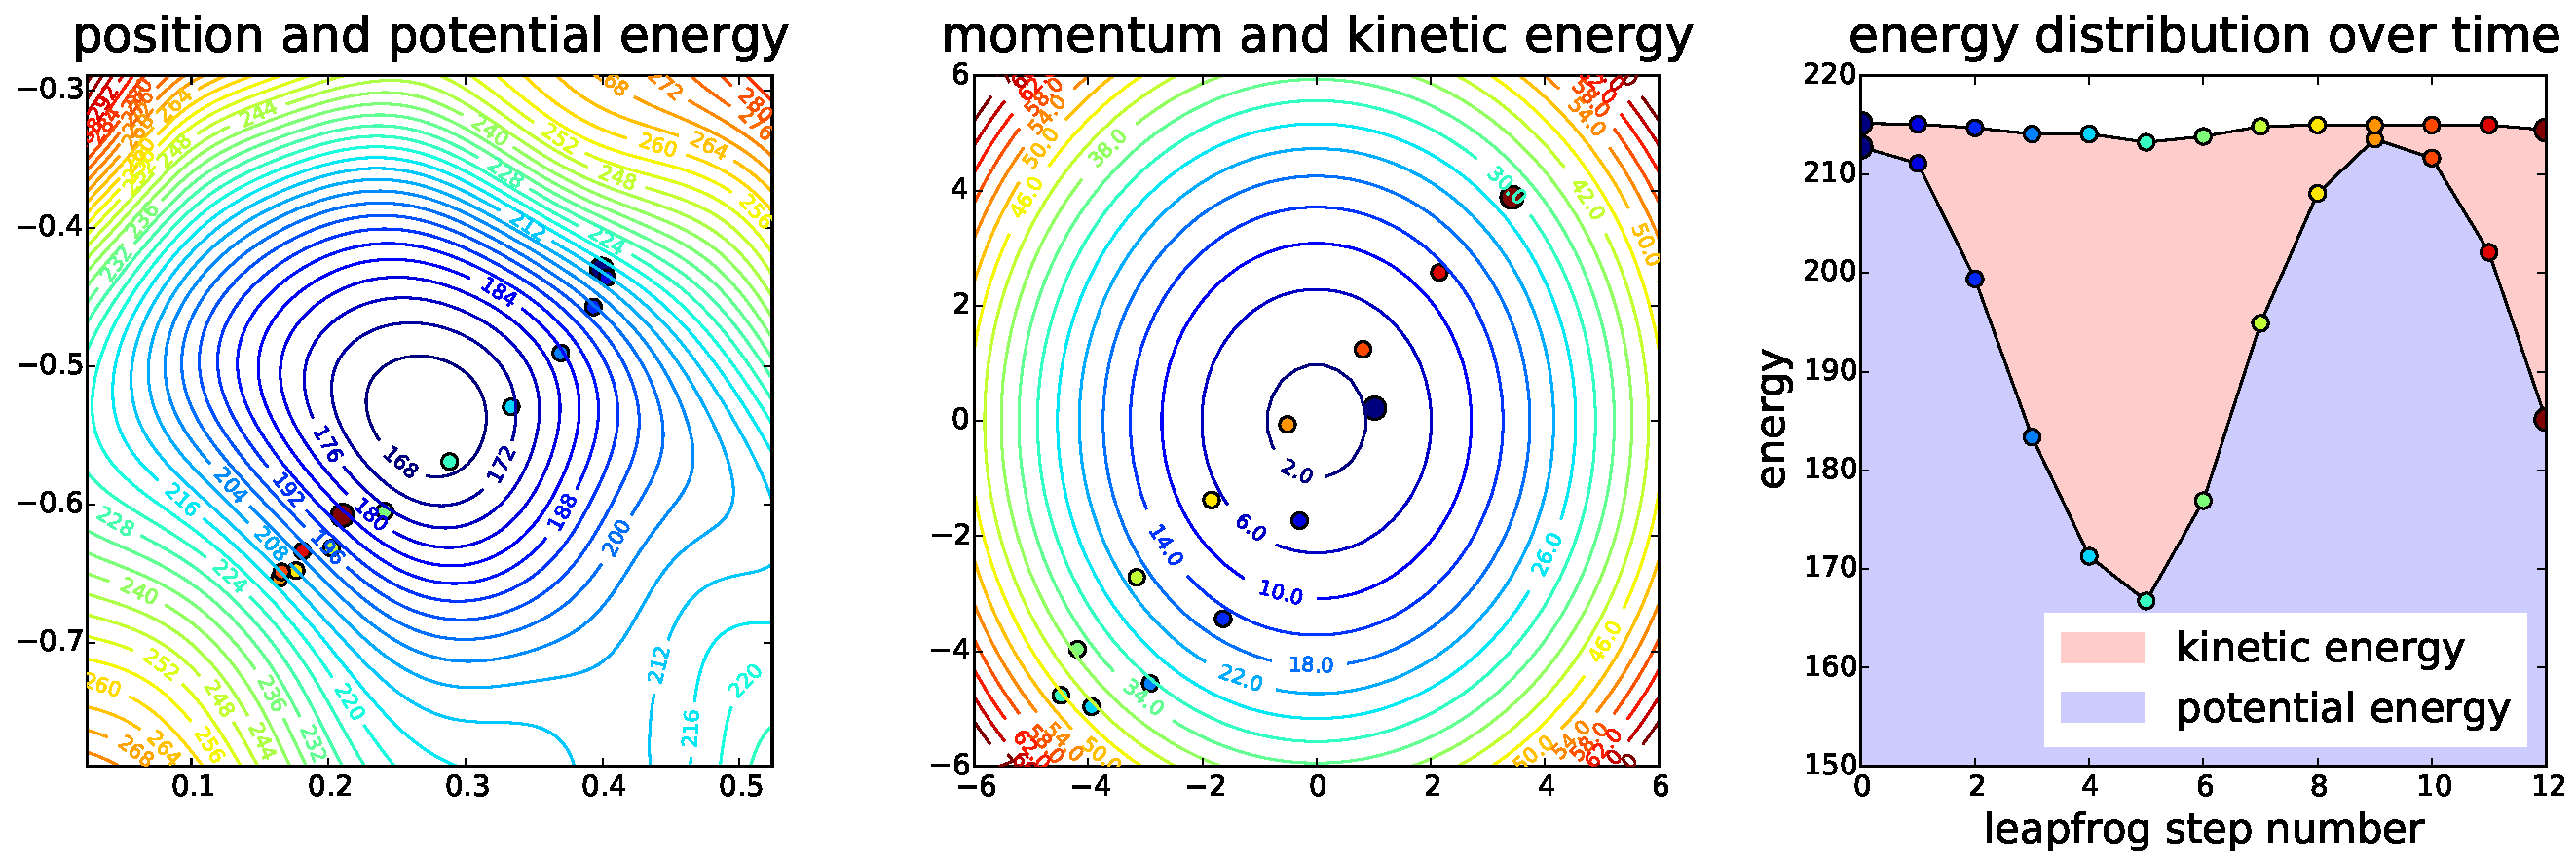
\includegraphics[width=\textwidth]{figures/hmc_motion_1hmc_12lf_presi.pdf}}
	\end{frame}	
	
	
	%------------------------------------------------
	\subsection{The algorithm} 
	%------------------------------------------------
	\begin{frame}
		\frametitle{The Hamiltonian Monte Carlo (HMC) algorithm}
		\centering		
		\includegraphics{figures/hmc_illustration_easy.tikz} % Acceptance step boils down to the difference in energies
		\\~\\
		\raggedright
		$\boldsymbol{\rightarrow}$ The constructed $(s_t)_{t \in \mathbb{N}}$ converges to $p(z|x) \cdot N(v|0, M)$ % The distributions introduced by the energies
	\end{frame}	

	%------------------------------------------------
	\subsection{Visualization} 
	%------------------------------------------------
	\begin{frame}
		\frametitle{Visualization of HMC}
		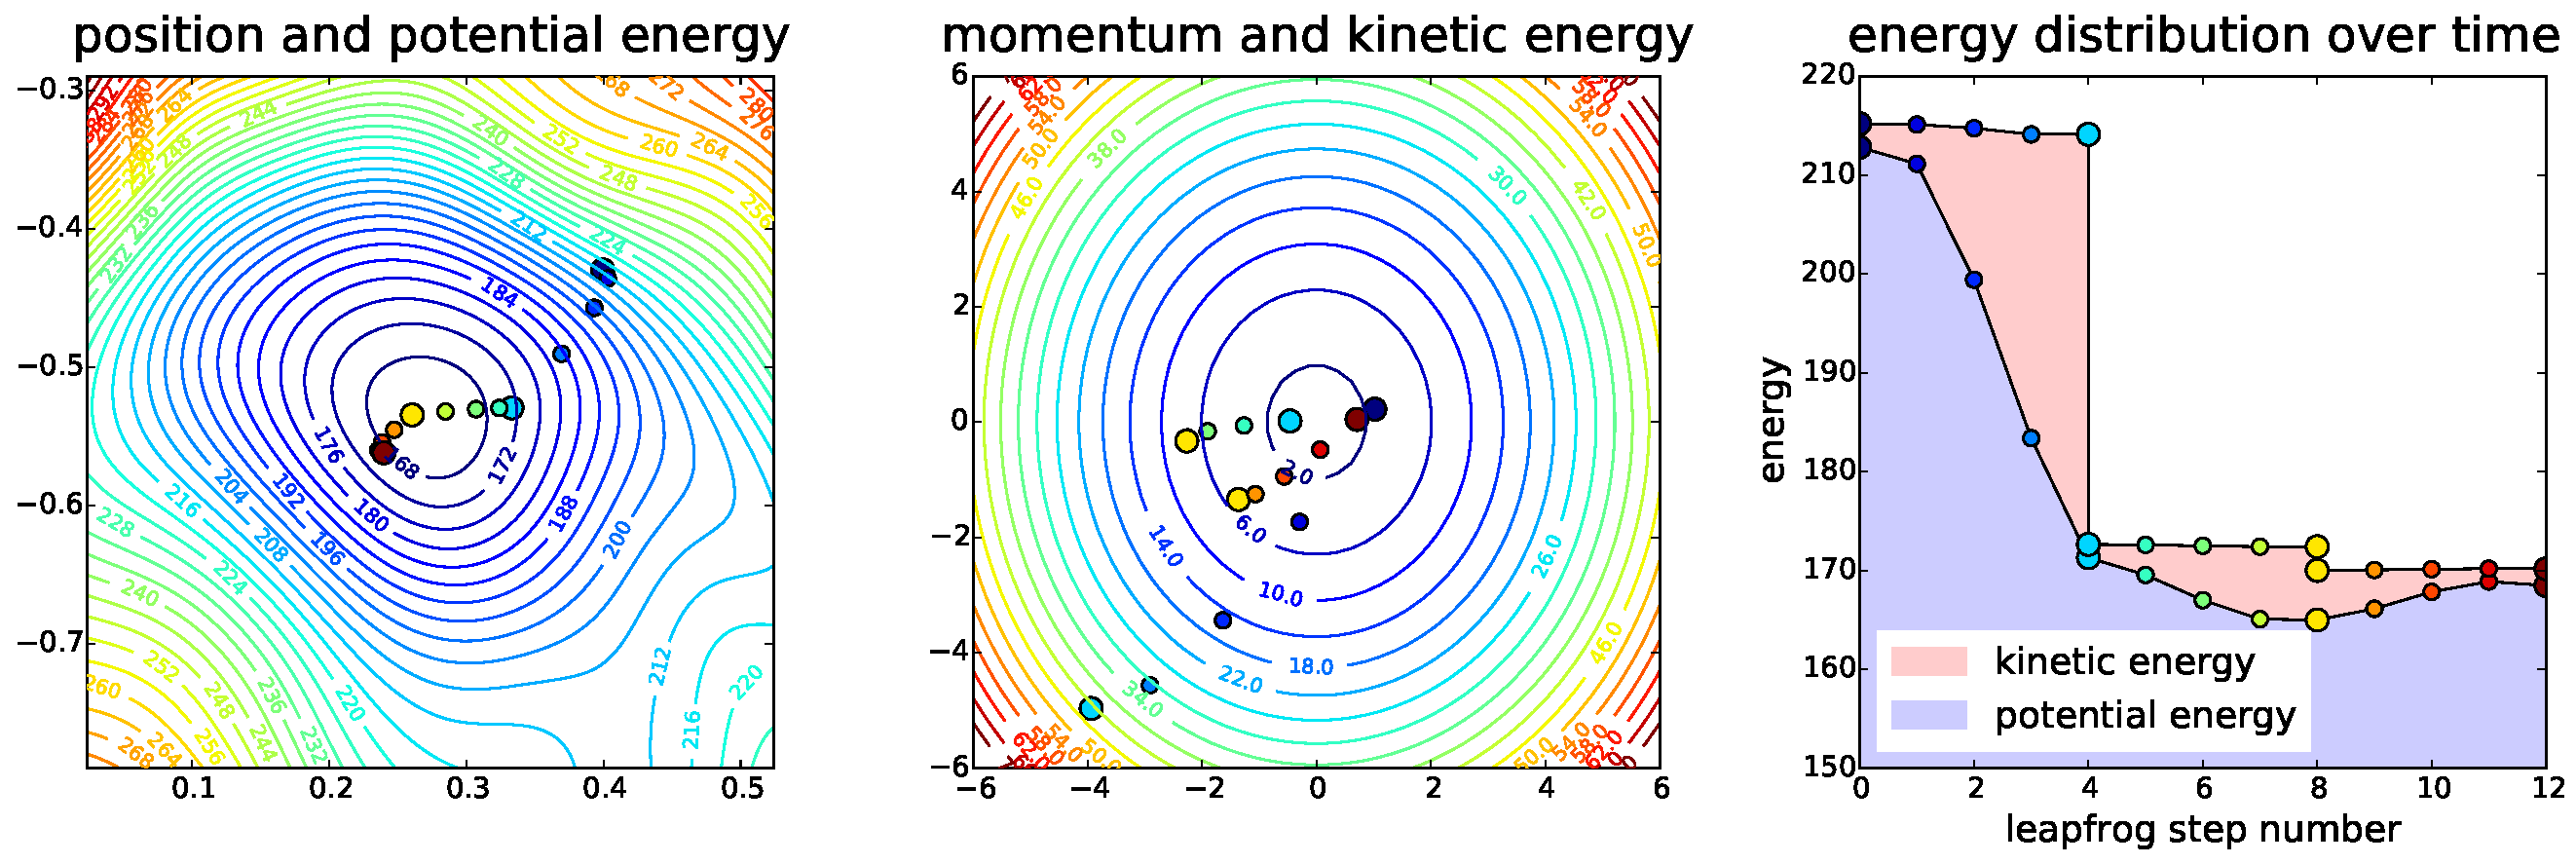
\includegraphics[width=\textwidth]{figures/hmc_motion_3hmc_04lf_presi.pdf}
		\\~\\
		$\boldsymbol{\rightarrow}$ Momentum resampling leads to changes in total energy\\~\\
		$\boldsymbol{\rightarrow}$ Hamiltonian Dynamics explore the state spaces
	\end{frame}
	

%------------------------------------------------
\section{Contributions}
%------------------------------------------------
% Salimans use HMC for this, BUT leave out the acceptance step -> wrong invariant distribution of Markov chain -> Convergence to something else
%			although probably initially similar
% However, turns out we can exploit the HMC algorithm's structure, to include the acceptance step
\begin{frame}
	\frametitle{Contributions}
	\begin{enumerate}
	\item Include the acceptance step of the HMC algorithm in VI \\~\\
	\item Integrate partial momentum updates into lower bound \\~\\
	\item Make the kinetic energy input-dependent
	\end{enumerate}
\end{frame}	
	
	%------------------------------------------------
	\subsection{Including the acceptance step} 
	%------------------------------------------------
	\begin{frame}  % Salimans left this out, since it can not be included for MCMC methods, where the state is just the variable of interest
		\frametitle{Including the acceptance step} % For HMC can exploit structure
		\tiny
		\mbox{}\hfill\raisebox{-\height}[0pt][0pt]{\includegraphics{figures/hmc_illustration_easy.tikz}}
 	 	\vspace*{-\baselineskip}
 	 	\small
 	 	\begin{flalign*}
			&f_{S_t|S_{t-1}, X}(s_t|s_{t-1}, x) &\\
			&\;=\sum_{a=0}^1 \int f_{S_t, A, V_{\textrm{sampled}}|S_{t-1}, X}(s_t, a, v|s_{t-1}, x) dv &\\
			&\;=\sum_{a=0}^1 \int f_{S_t|A, V_{\textrm{sampled}}, S_{t-1}, X}(s_t| a, v, s_{t-1}, x) &\\
			&\qquad\qquad\cdot \mathbb{P}(A = a|V_{\textrm{sampled}} = v, S_{t-1} = s_{t-1}, x) &\\
			&\qquad\qquad \cdot f_{V_{\textrm{sampled}}|S_{t-1}, X}(v|s_{t-1}, x) dv&
		\end{flalign*}
		\\~\\~\\
		$\boldsymbol{\rightarrow}$ With acceptance step: Asymptotic convergence is guaranteed
	\end{frame}	

	%------------------------------------------------
	\subsection{Partial momentum updates} 
	%------------------------------------------------
	\begin{frame}
		\frametitle{Partial momentum updates}
		In resampling step: Use weighted sum of current momentum and newly sampled momentum \\~\\ % instead of completely new sample
		\uncover<2->{Effects:\\ \begin{itemize}
		\item Particle tends to maintain its direction in the resampling step \\~\\
		\item Avoids random walk behaviour \\~\\
		\item Reduction of total energy is slower \\~\\
		\end{itemize}
		$\boldsymbol{\rightarrow}$ For sampling with HMC: Shown to be beneficial for short trajectories}  % Can be learnt as part of the model
	\end{frame}	
	% Gedanken erklären

	%------------------------------------------------
	\subsection{Adaptive kinetic energy} 
	%------------------------------------------------
	\begin{frame}
		\frametitle{Adaptive kinetic energy}
		\textbf{Idea}: Allow mass matrix $M$ in the kinetic energy to depend on $x$ \\~\\  % e.g. through a neural network
		\uncover<2->{\textbf{Relevance}: For trajectories of Hamiltonian Dynamics:\\ $\qquad\qquad$Change of mass matrix $\iff$ Rescaling of $z$-space\\
		\begin{itemize}
		\item Scaling too small $\boldsymbol{\rightarrow}$ Large numerical errors \\~\\
		\item Scaling too large $\boldsymbol{\rightarrow}$ Slow exploration of the state space \\~\\
		\end{itemize}
		$\boldsymbol{\rightarrow}$ Input-dependent kinetic energy should improve convergence}
	\end{frame}	
	
%------------------------------------------------
\section{Experimental results}
%------------------------------------------------

	%------------------------------------------------
	\subsection{Binarized MNIST dataset} 
	%------------------------------------------------
	\begin{frame}
		\frametitle{Experimental setup}
		Variational Auto-Encoders on stochastically binarized MNIST digits \\~\\
		\uncover<2->{
		\mbox{}\hfill\raisebox{-\height}[0pt][0pt]{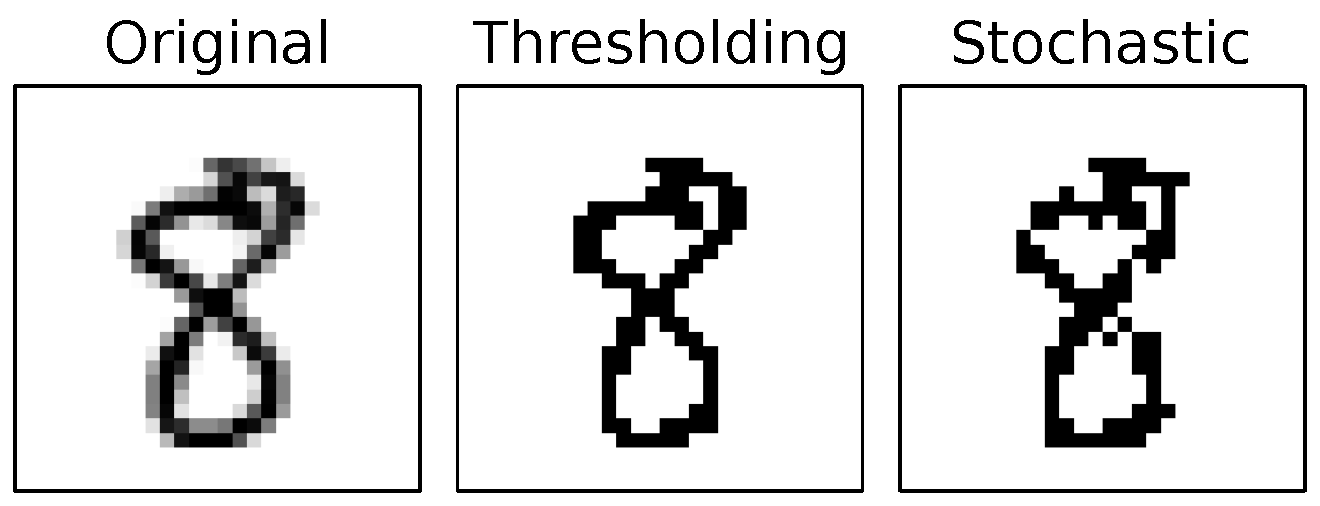
\includegraphics[width=.5\linewidth]{figures/binarization_example_header.pdf}}
 	 	\vspace*{-\baselineskip}
 	 	\\	~\\
		\begin{itemize}
		\item \lenitem{Binarization: Want bilevel image to match Bernoulli modelling assumption\\}}
		\uncover<3->{ 
		\item Stochastic binarization: Randomly set pixel to 1 with probability given by its pixel value\\~\\
		\item Effectively much larger dataset; similar effect to dropout regularization}
		\end{itemize}
	\end{frame}
	
	%------------------------------------------------
	\subsection{Model comparisons} 
	%------------------------------------------------
	\begin{frame}
		\frametitle{Experimental results}
		\centering
		\resizebox{\columnwidth}{!}{% \begin{tabular}{@{}l@{}c@{}r@{$\;\;\;$}r@{}c@{}r@{$\;\;$}r@{}c@{}r@{}}
% \toprule
% & \phantom{abc}  & \multicolumn{2}{c}{CPU} & \phantom{abc} & \multicolumn{2}{c}{GPU} & \phantom{abc}  & \tn 
% \cmidrule{3-4} \cmidrule{6-7} 
% $r_{z}$ && $e_{rel}$  & $t$ && $e_{rel}$  & $t$ && $M$\tn 
% &&  [$10^{-5}$]  & [ms] && [$10^{-5}$]  & [ms]&& [MB]\tn 

\begin{tabular}{lrrrrrrrr}
\toprule
Name & \#HMC & \#LF & Partial & $M$ & Accept & $-\mathcal{L}_{\textrm{aux}}$ & $- \log(p(x)) \approx$ \tn 
\midrule
\rowcolor{red!20}
Basic VI & 0 & 0 & - & - & - & 92.35 & 88.27 \tn 
\rowcolor{red!20}
HMCVI 1 & 1 & 12 & - & Global & - & 89.77 & 87.77 \tn 
\rowcolor{red!20}
HMCVI 2 & 2 & 6 & - & Global & - & 89.83 & 87.53 \tn 
\rowcolor{red!20}
HMCVI 3 & 3 & 4 & - & Global & - & 90.24 & 87.56 \tn 
HMCVI 4 & 3 & 4 & Yes & Global & - & 90.15 & 87.49 \tn
HMCVI 5 & 3 & 4 & - & NN & - & 90.23 & 87.30 \tn 
HMCVI 6 & 3 & 4 & Yes & NN & - & 89.72 & 87.44 \tn 
HMCVI 7 & 3 & 4 & - & Global & Yes & 91.40 & 87.28 \tn
HMCVI 8 & 3 & 4 & - & NN & Yes & 91.38 & 87.20 \tn 
\bottomrule
\end{tabular}
}
		\raggedright
		\\~\\~\\
		$\boldsymbol{\rightarrow}$ VI with HMC outperforms basic VI \\~\\
		\textcolor{white}{$\boldsymbol{\rightarrow}$ Extensions to the HMC algorithm improve the performance \\~\\
		$\boldsymbol{\rightarrow}$ Acceptance step improves the NLL}
	\end{frame}
	
	\begin{frame}[noframenumbering]
		\frametitle{Experimental results}
		\centering
		\resizebox{\columnwidth}{!}{% \begin{tabular}{@{}l@{}c@{}r@{$\;\;\;$}r@{}c@{}r@{$\;\;$}r@{}c@{}r@{}}
% \toprule
% & \phantom{abc}  & \multicolumn{2}{c}{CPU} & \phantom{abc} & \multicolumn{2}{c}{GPU} & \phantom{abc}  & \tn 
% \cmidrule{3-4} \cmidrule{6-7} 
% $r_{z}$ && $e_{rel}$  & $t$ && $e_{rel}$  & $t$ && $M$\tn 
% &&  [$10^{-5}$]  & [ms] && [$10^{-5}$]  & [ms]&& [MB]\tn 

\begin{tabular}{lrrrrrrrr}
\toprule
Name & \#HMC & \#LF & Partial & $M$ & Accept & $-\mathcal{L}_{\textrm{aux}}$ & $- \log(p(x)) \approx$ \tn 
\midrule
Basic VI & 0 & 0 & - & - & - & 92.35 & 88.27 \tn 
HMCVI 1 & 1 & 12 & - & Global & - & 89.77 & 87.77 \tn 
HMCVI 2 & 2 & 6 & - & Global & - & 89.83 & 87.53 \tn 
\rowcolor{red!20}
HMCVI 3 & 3 & 4 & - & Global & - & 90.24 & 87.56 \tn 
\rowcolor{red!20}
HMCVI 4 & 3 & 4 & Yes & Global & - & 90.15 & 87.49 \tn
\rowcolor{red!20}
HMCVI 5 & 3 & 4 & - & NN & - & 90.23 & 87.30 \tn 
\rowcolor{red!20}
HMCVI 6 & 3 & 4 & Yes & NN & - & \textbf{89.72} & 87.44 \tn 
HMCVI 7 & 3 & 4 & - & Global & Yes & 91.40 & 87.28 \tn
HMCVI 8 & 3 & 4 & - & NN & Yes & 91.38 & 87.20 \tn 
\bottomrule
\end{tabular}
}
		\raggedright
		\\~\\~\\
		$\boldsymbol{\rightarrow}$ VI with HMC outperforms basic VI \\~\\
		$\boldsymbol{\rightarrow}$ Extensions to the HMC algorithm improve the performance \\~\\
		\textcolor{white}{$\boldsymbol{\rightarrow}$ Acceptance step improves the NLL}
	\end{frame}
	
	\begin{frame}[noframenumbering]
		\frametitle{Experimental results}
		\centering
		\resizebox{\columnwidth}{!}{% \begin{tabular}{@{}l@{}c@{}r@{$\;\;\;$}r@{}c@{}r@{$\;\;$}r@{}c@{}r@{}}
% \toprule
% & \phantom{abc}  & \multicolumn{2}{c}{CPU} & \phantom{abc} & \multicolumn{2}{c}{GPU} & \phantom{abc}  & \tn 
% \cmidrule{3-4} \cmidrule{6-7} 
% $r_{z}$ && $e_{rel}$  & $t$ && $e_{rel}$  & $t$ && $M$\tn 
% &&  [$10^{-5}$]  & [ms] && [$10^{-5}$]  & [ms]&& [MB]\tn 

\begin{tabular}{lrrrrrrrr}
\toprule
Name & \#HMC & \#LF & Partial & $M$ & Accept & $-\mathcal{L}_{\textrm{aux}}$ & $- \log(p(x)) \approx$ \tn 
\midrule
Basic VI & 0 & 0 & - & - & - & 92.35 & 88.27 \tn 
HMCVI 1 & 1 & 12 & - & Global & - & 89.77 & 87.77 \tn 
HMCVI 2 & 2 & 6 & - & Global & - & 89.83 & 87.53 \tn 
\rowcolor{red!20}
HMCVI 3 & 3 & 4 & - & Global & - & 90.24 & 87.56 \tn 
HMCVI 4 & 3 & 4 & Yes & Global & - & 90.15 & 87.49 \tn
\rowcolor{red!20}
HMCVI 5 & 3 & 4 & - & NN & - & 90.23 & 87.30 \tn 
HMCVI 6 & 3 & 4 & Yes & NN & - & \textbf{89.72} & 87.44 \tn 
\rowcolor{red!20}
HMCVI 7 & 3 & 4 & - & Global & Yes & 91.40 & 87.28 \tn
\rowcolor{red!20}
HMCVI 8 & 3 & 4 & - & NN & Yes & ??? & \textbf{???} \tn 
\bottomrule
\end{tabular}
}
		\raggedright
		\\~\\~\\
		$\boldsymbol{\rightarrow}$ VI with HMC outperforms basic VI \\~\\
		$\boldsymbol{\rightarrow}$ Extensions to the HMC algorithm improve the performance \\~\\
		$\boldsymbol{\rightarrow}$ Acceptance step improves the NLL
	\end{frame}
			
%------------------------------------------------
\section{Future work}
%------------------------------------------------
\begin{frame}
	\frametitle{Future work}
	\begin{itemize}
	\item More flexible reverse model \\~\\
	\item Understand role of the auxiliary reverse model \\~\\
	\item Speed up algorithm \\~\\
	\item Allow other parameters to be input-dependent
	\end{itemize}
\end{frame}
	
%------------------------------------------------
\begin{frame}[plain]
\Huge{\centerline{Thank you for your attention}}
\end{frame}
%------------------------------------------------

%------------------------------------------------
\begin{frame}[plain]
\frametitle{References}
\printbibliography{}
\end{frame}

\section{Extra slides}

\begin{frame}[noframenumbering]
	\frametitle{Visualizations of HMC (2)}
	\centering
	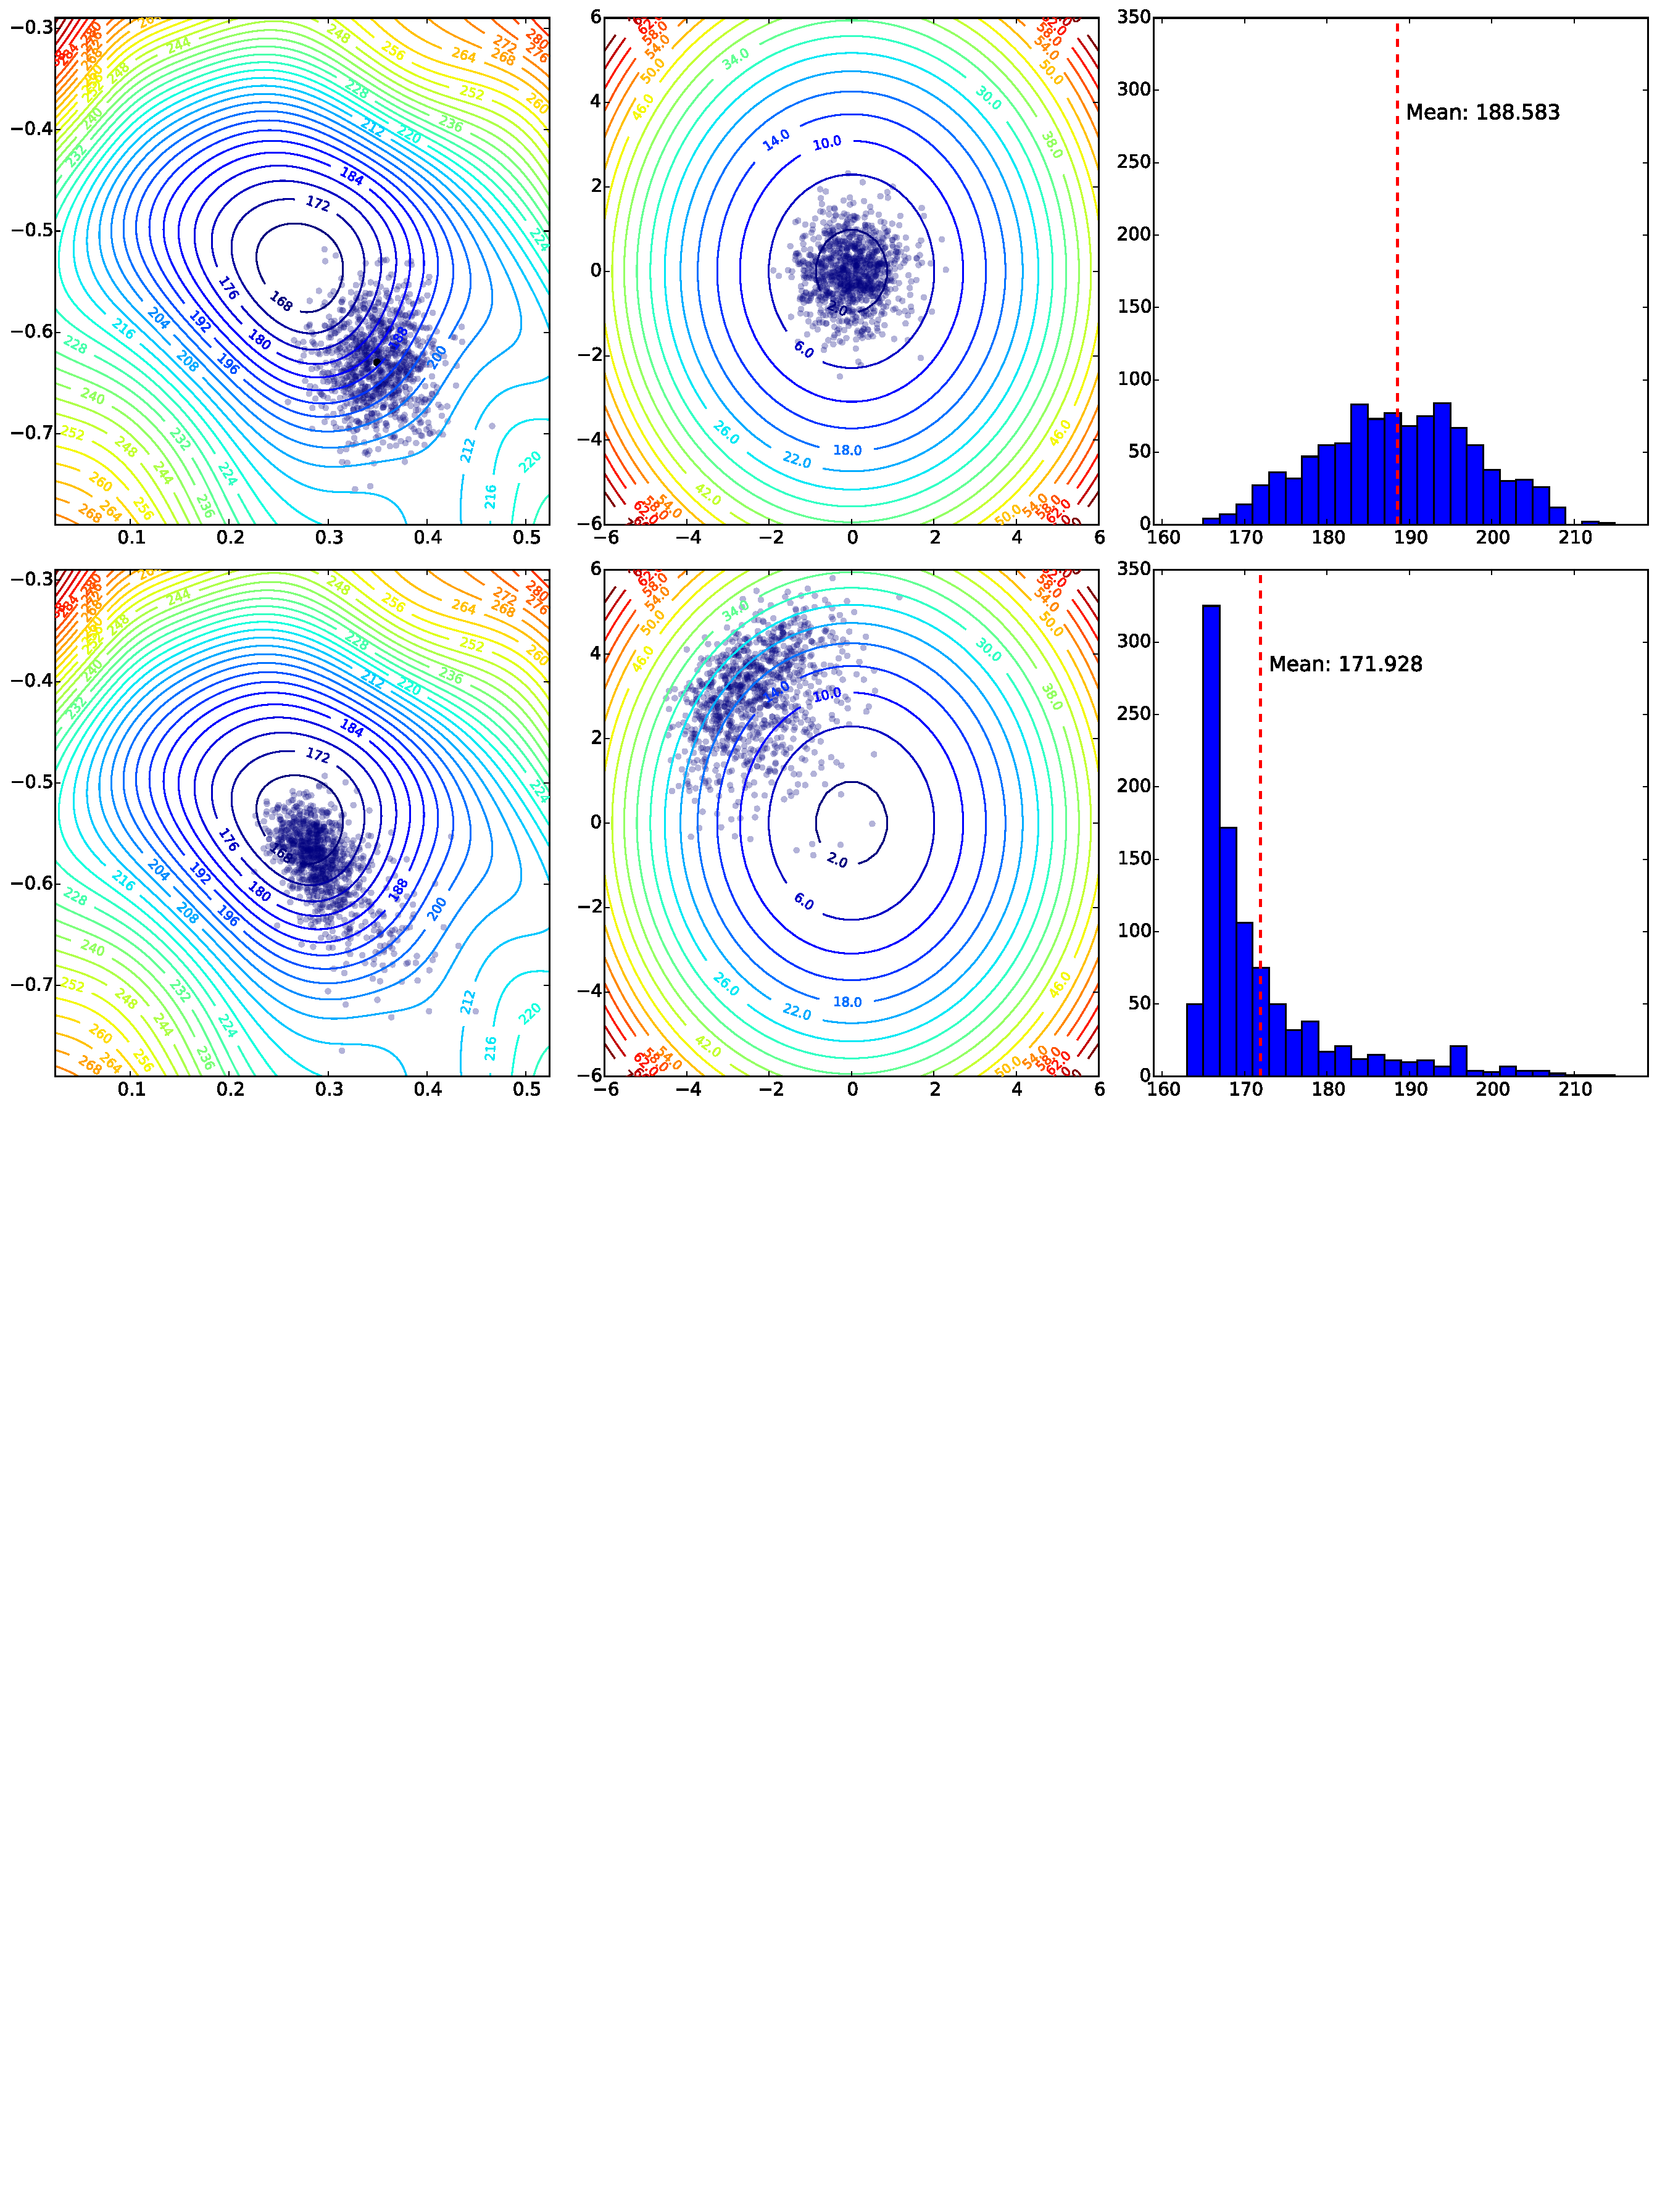
\includegraphics[width=\textwidth]{figures/hmcvi_distrib_example_top.pdf}
\end{frame}	

\begin{frame}[noframenumbering]
	\frametitle{Potential energy of VAEs}
	\centering
	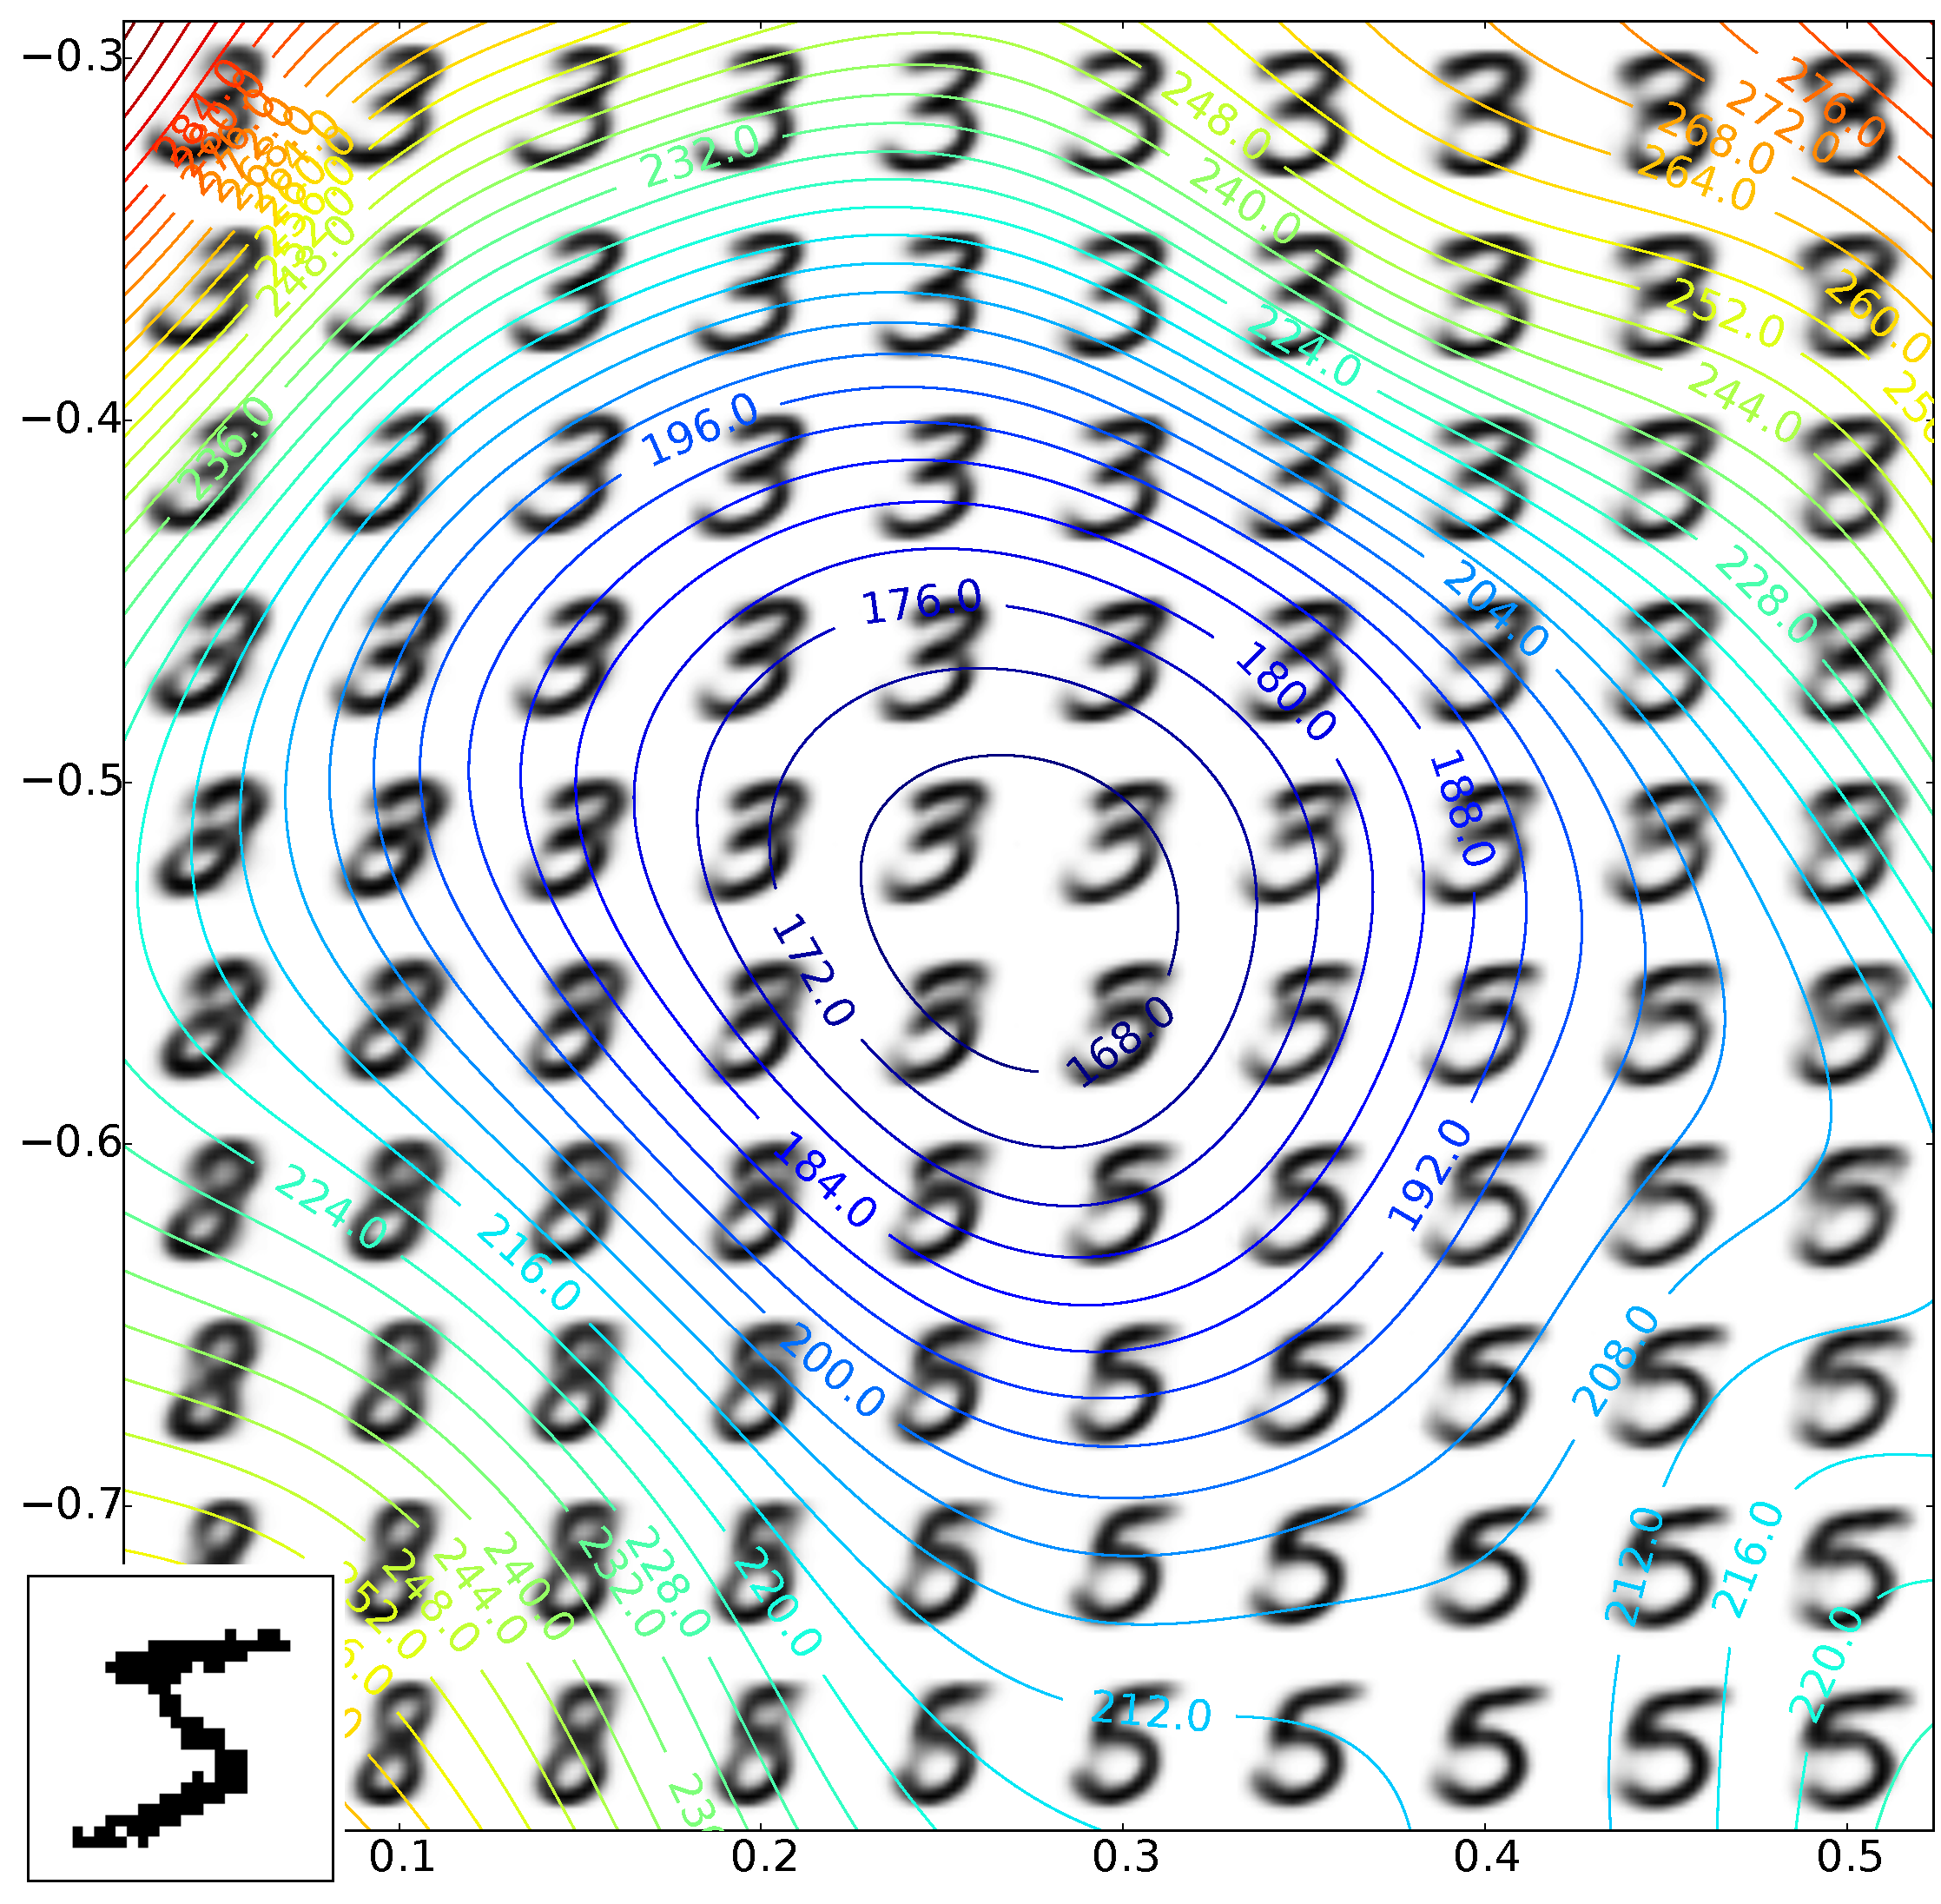
\includegraphics[width=0.7\textwidth]{figures/vae_pot_energy_example_with_inset.pdf}
\end{frame}

\begin{frame}[noframenumbering]
	\frametitle{Learnt latent representation of training data}
	\centering
	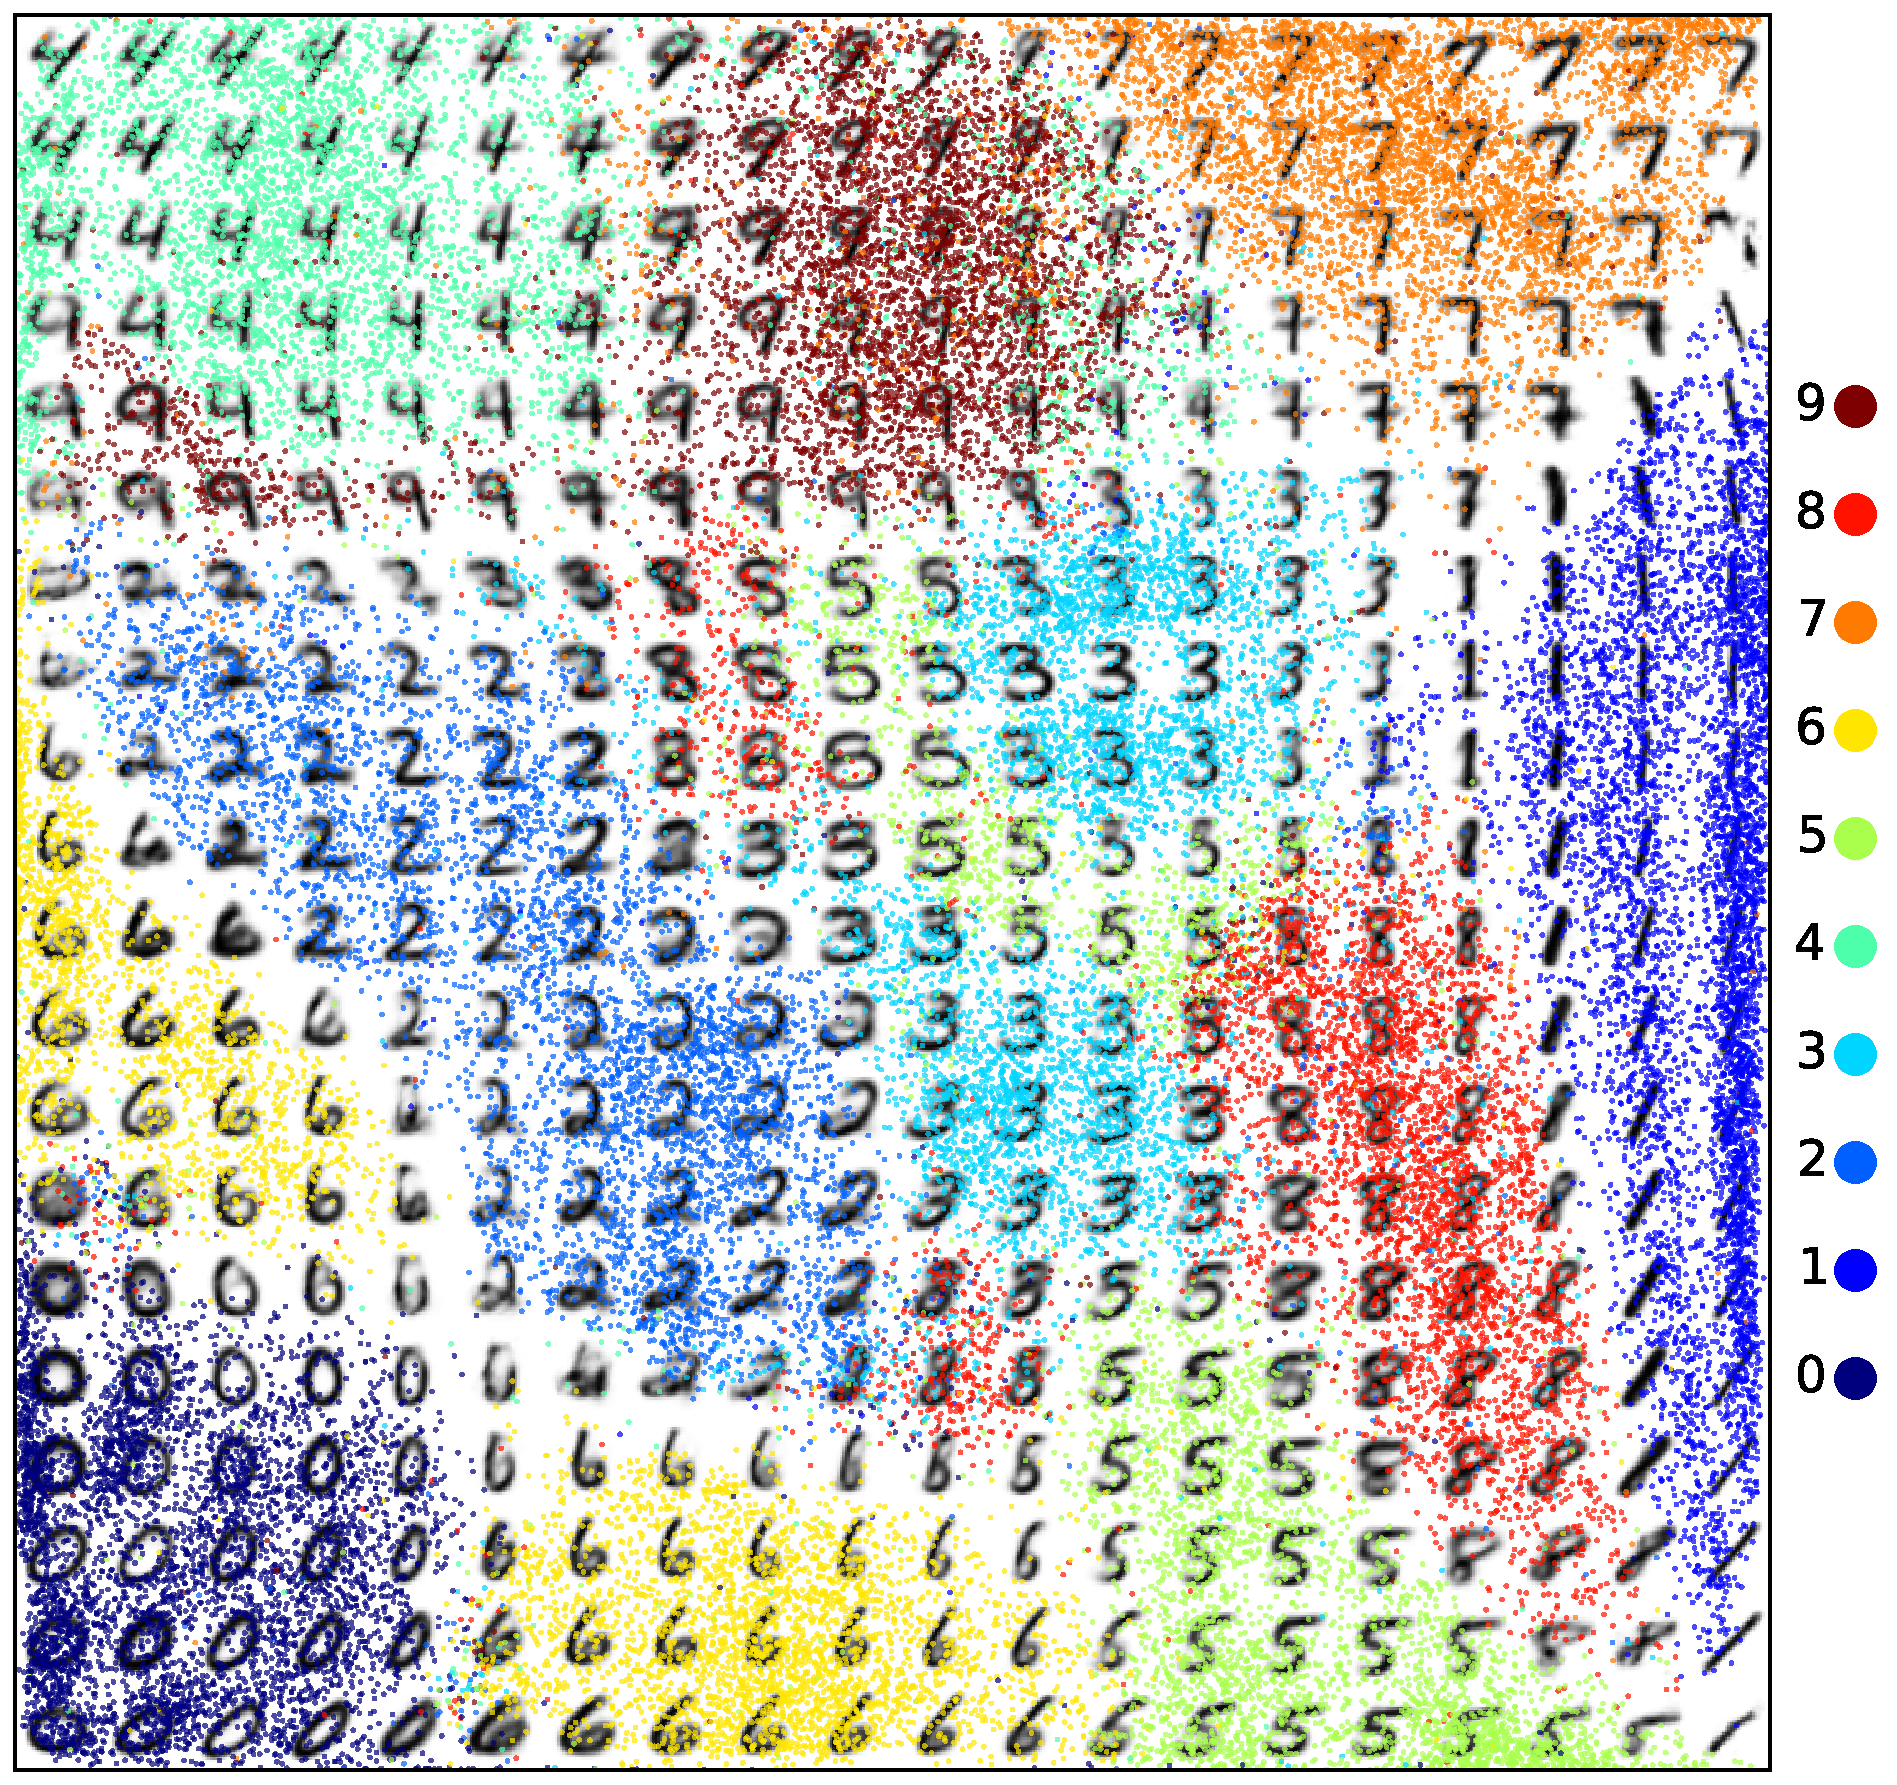
\includegraphics[width=0.7\textwidth]{figures/learned_representation_train_points_small.pdf}
\end{frame}

\end{document} 